\documentclass[e4_tp1_main.tex]{subfiles}
\begin{document}

\section{Funcionamiento real de una fuente DC/DC}

Combinando el circuito de disparo con la fuente diseñada en la sección previa, el circuito resulta:

\begin{figure}[H]
\centering

\includegraphics[width=1\linewidth]{Imagenes/Punto3/Circuito3.png}
\end{figure}

\subsection*{a) Curvas Simuladas}

Se toman por un lado las curvas correspondientes a la conmutación del transistor.

\begin{figure}[H]
\centering
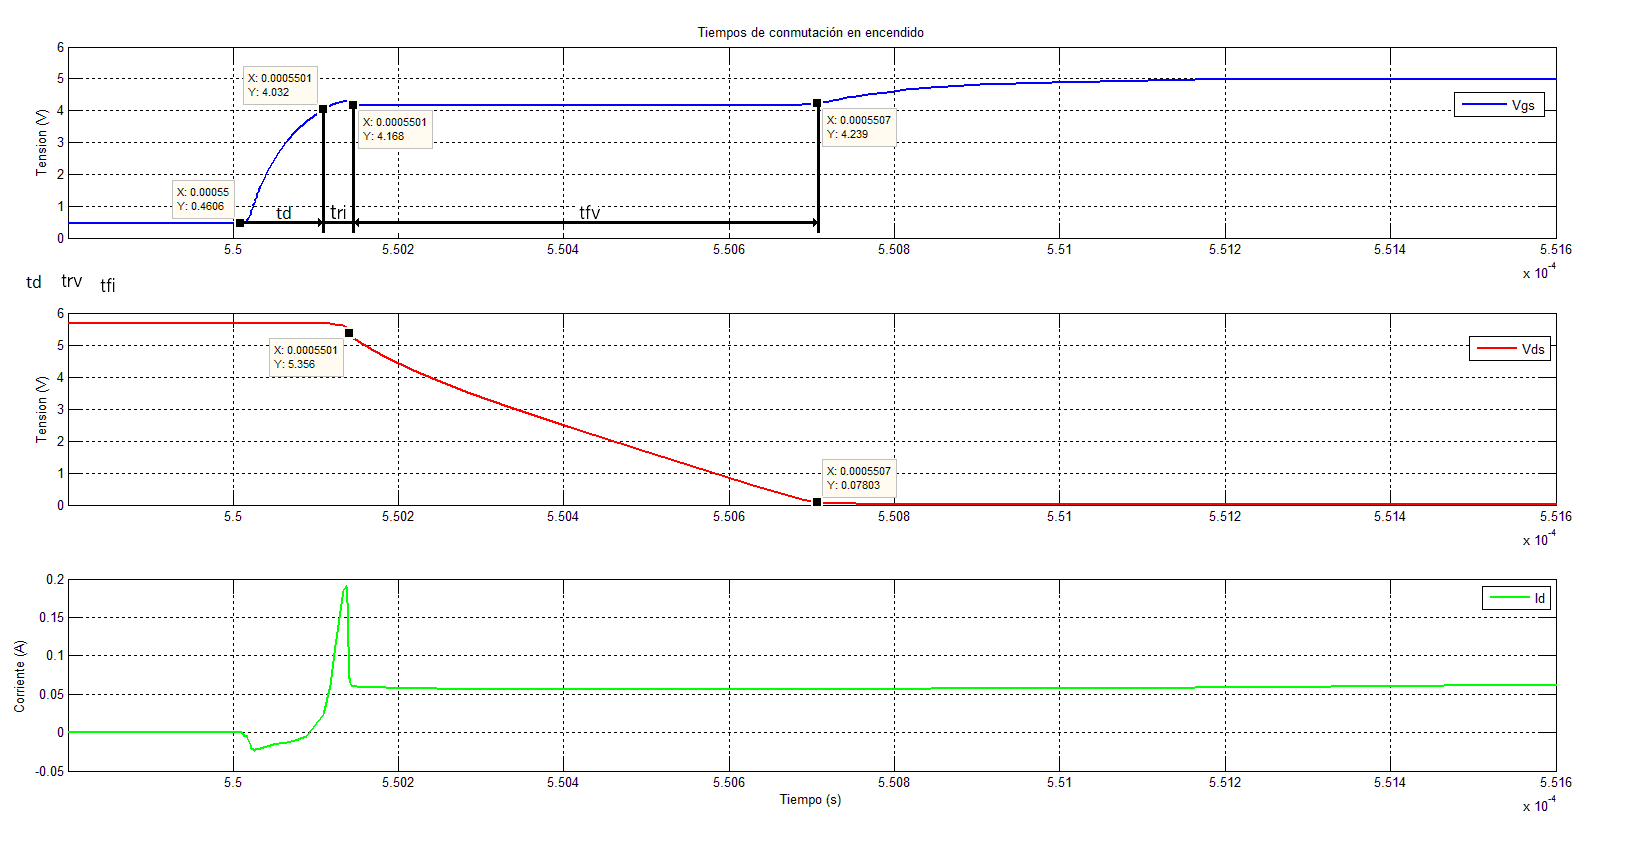
\includegraphics[width=1\linewidth]{Imagenes/Punto3/tiempos_encendidoX.png}
\caption{Curvas de encendido simulado}
\end{figure}

De donde se tabulan los tiempos de encendido:

\[
t_d(ON) = 98nS \hspace{2cm} t_{ri} = 27nS \hspace{2cm} t_{fv} = 556nS
\]

\subsubsection*{1- Comparaciones y observaciones}

El comportamiento de dichas curvas resulta el mismo desarrollado en la sección 1. Cuando el canal empieza a conducir, la tensión en sentido opuesto generada en la bobina hace subir la tensión sobre el drain, produciendo que el diodo conduzca en directa durante un breve tiempo y luego, al pasar a estar en inversa (cuando empieza a caer en forma efectiva la $V_{ds}$), se observa el pico de corriente $I_{rr}$. Luego, mientras el canal conduce, la corriente a través de éste es igual a la de la bobina.\par
En este caso, los tiempos de conmutación de encendido resultan mayores en comparación al caso del circuito de disparo de la sección 1. Esto se debe a que el valor de $V_{ds}$ cuando el canal no conduce es de $5V$, contra los $50V$ del primer caso. Debido a esto, la capacidad $C_{iss} = C_{gd1} + C_{gs}$, de acuerdo a la hoja de datos, es mayor, por lo que los tiempos de carga resultarán mayores.

\begin{figure}[H]
\centering
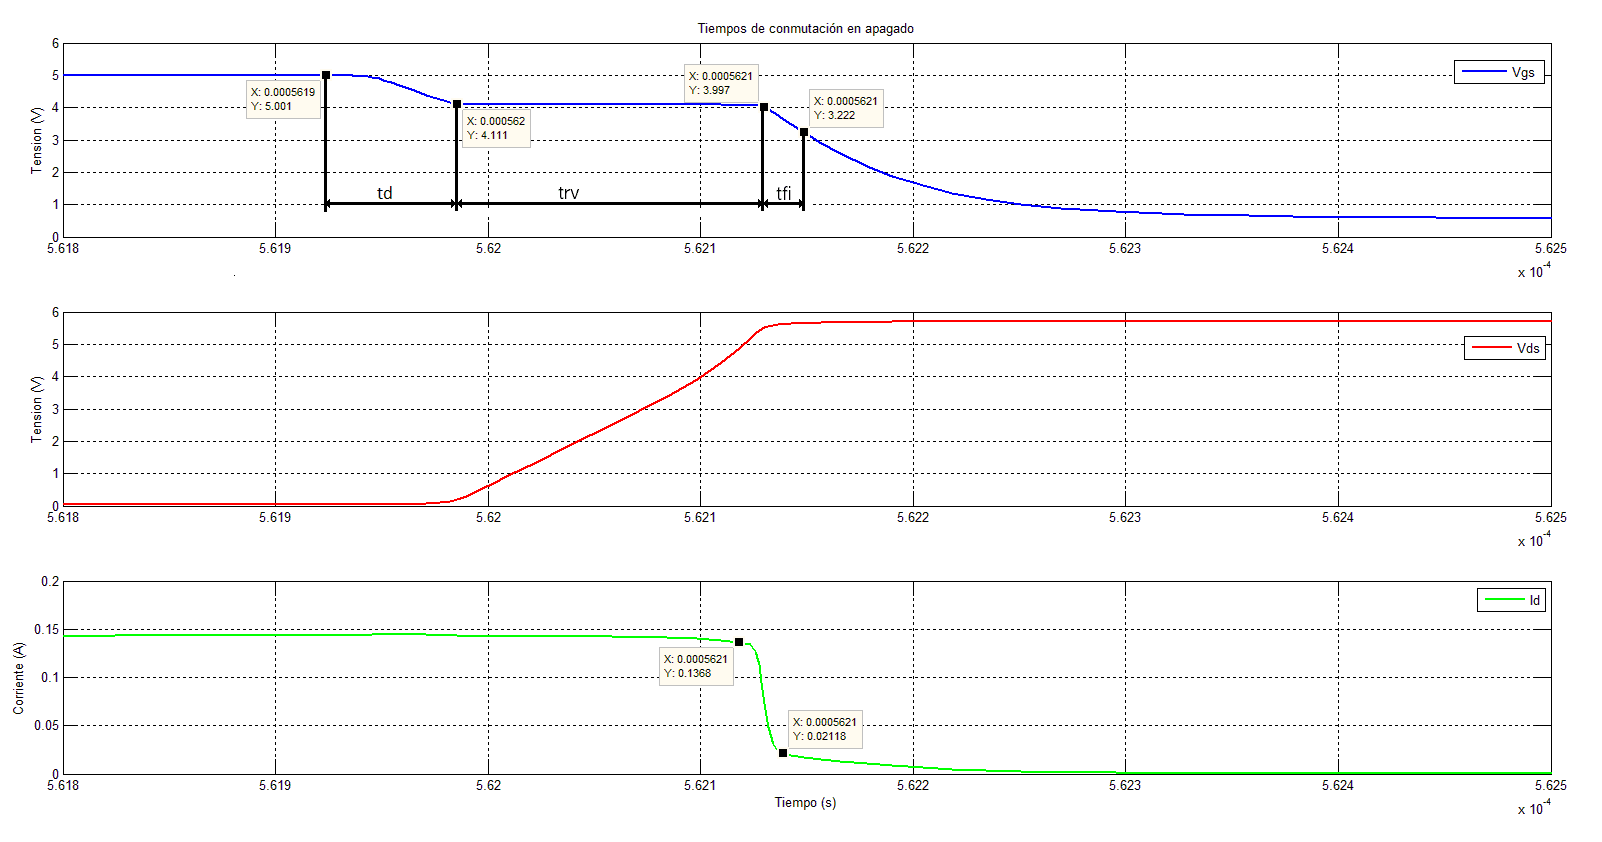
\includegraphics[width=1\linewidth]{Imagenes/Punto3/tiempos_apagadoX.png}
\caption{Curvas de apagado simulado}
\end{figure}

De donde se tabulan los tiempos de apagado:

\[
t_d(OFF) = 56nS \hspace{2cm} t_{rv} = 137nS \hspace{2cm} t_{fi} = 8nS 
\]

\subsubsection*{1- Comparaciones y observaciones}

El comportamiento de las curvas de apagado resulta similar al desarrollado en la sección 1. En este caso, los tiempos de conmutación son más rápidos que en el circuito de disparo original.
\par

Por otro lado, se toman las curvas de las tensiones y corrientes de los diferentes elementos:

\begin{figure}[H]
\centering
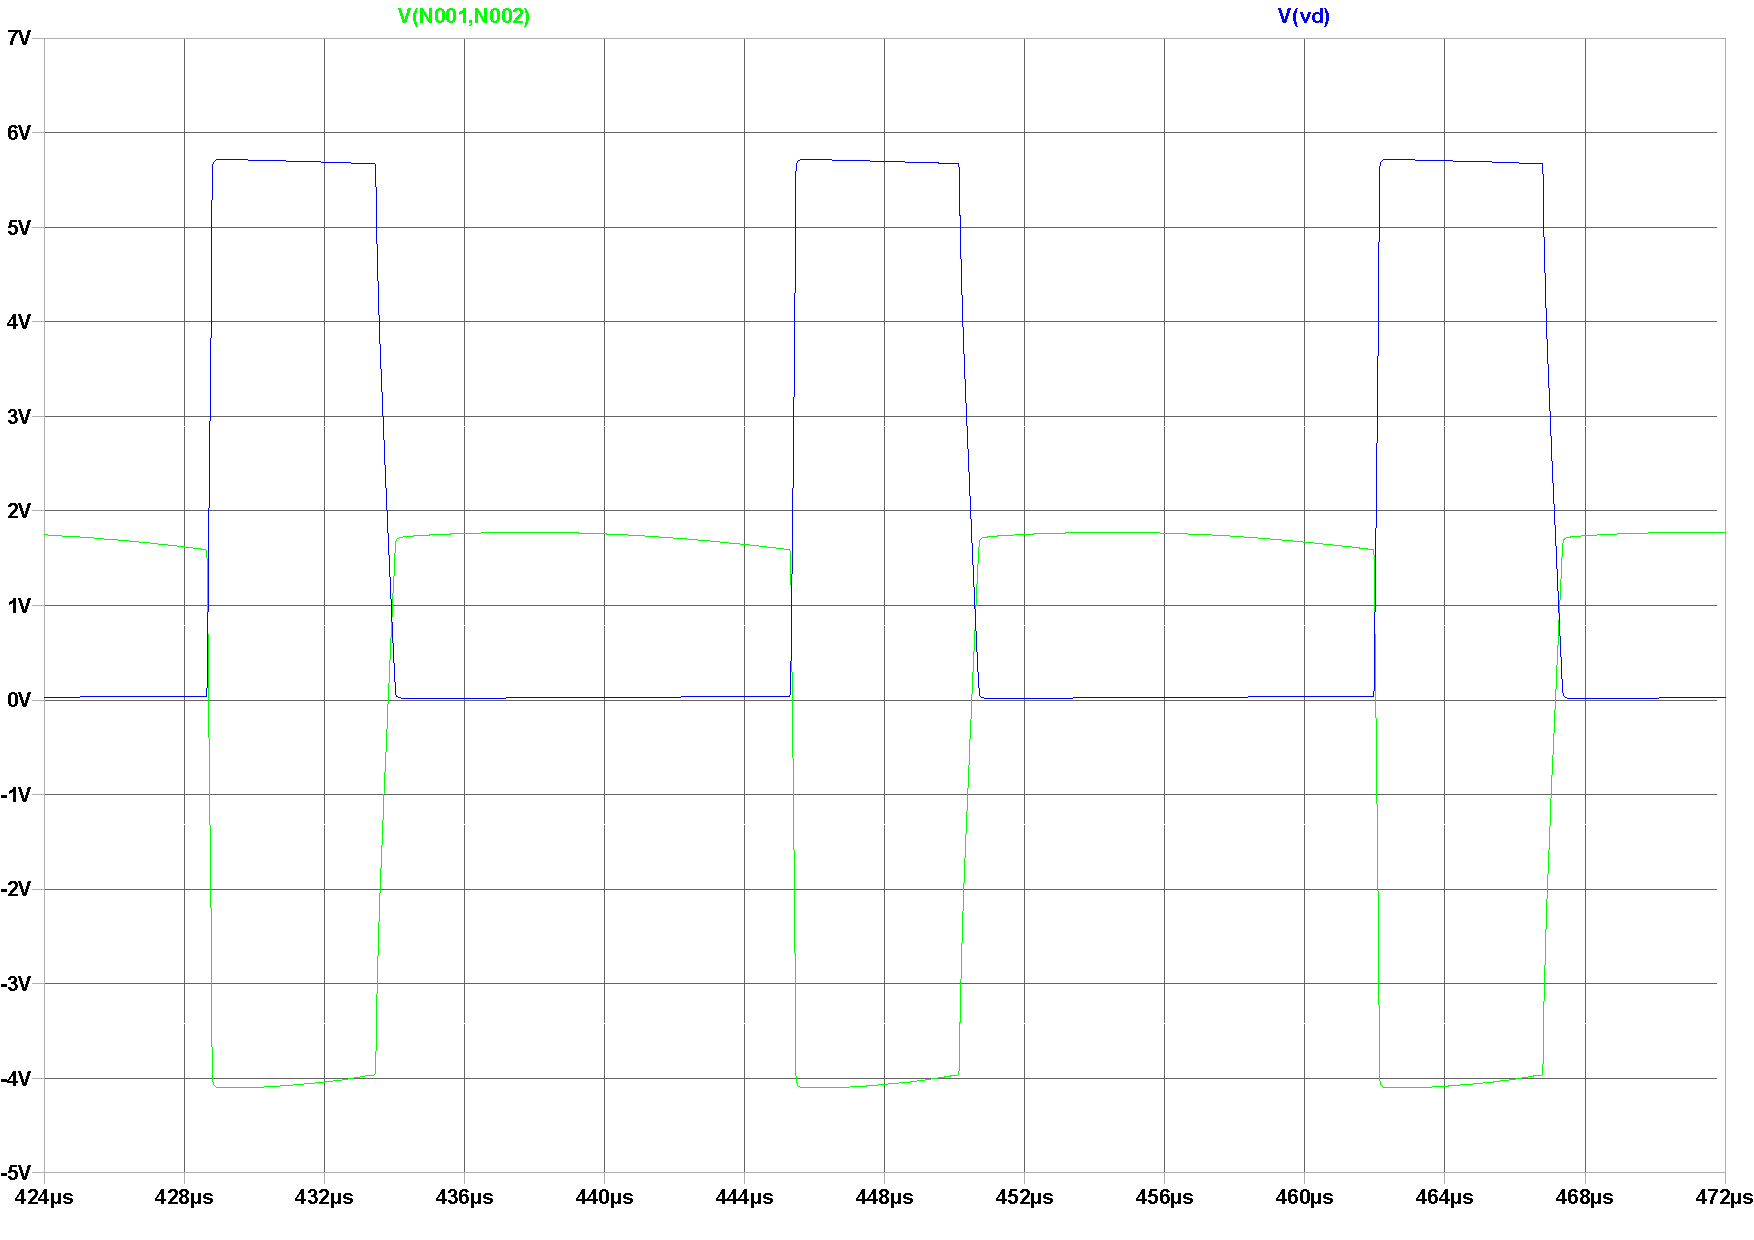
\includegraphics[width=0.8\linewidth]{Imagenes/Punto3/Sw-VL.pdf}
\caption{Simulación Sw(azul) y VL(verde)}
\end{figure}

\begin{figure}[H]
\centering
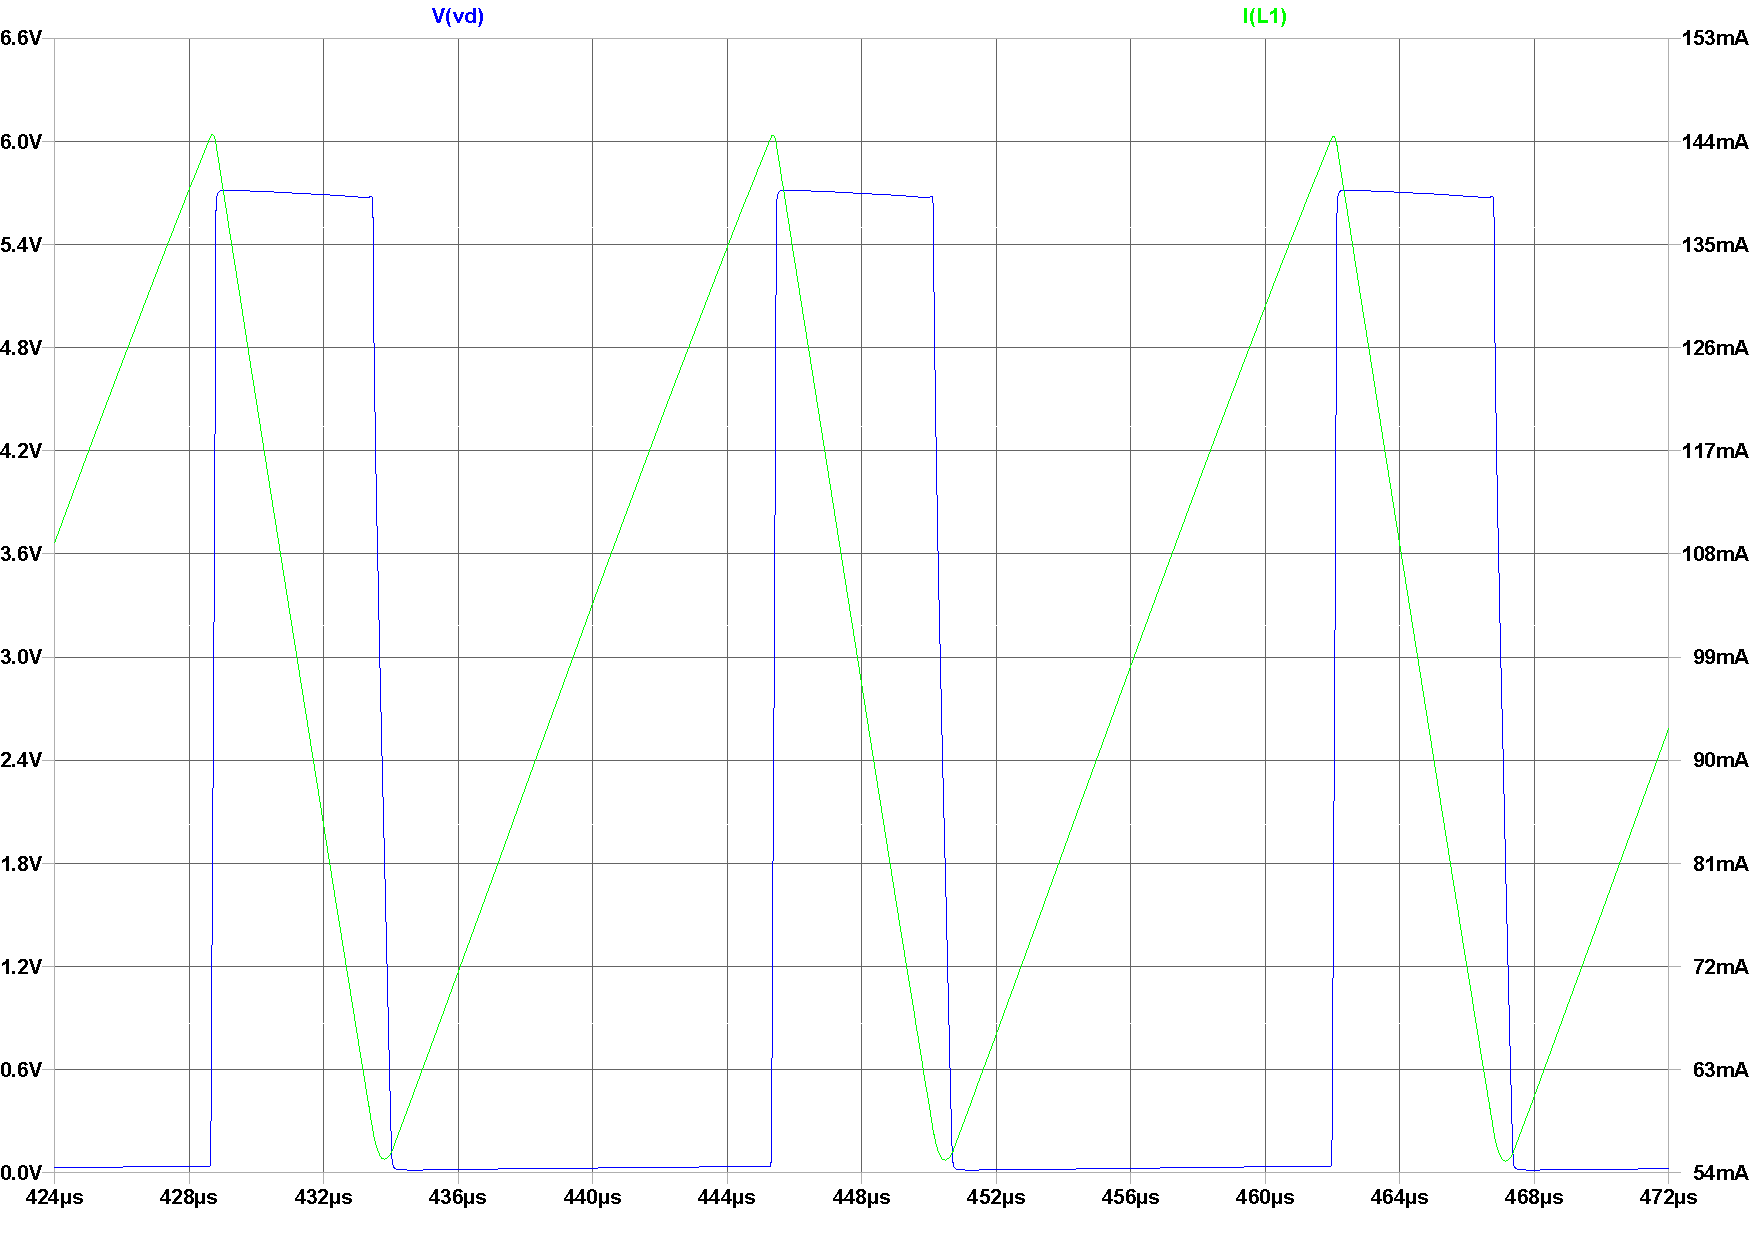
\includegraphics[width=0.8\linewidth]{Imagenes/Punto3/Sw-IL.pdf}
\caption{Simulación Sw(azul) y IL(verde)}
\end{figure}

\begin{figure}[H]
\centering
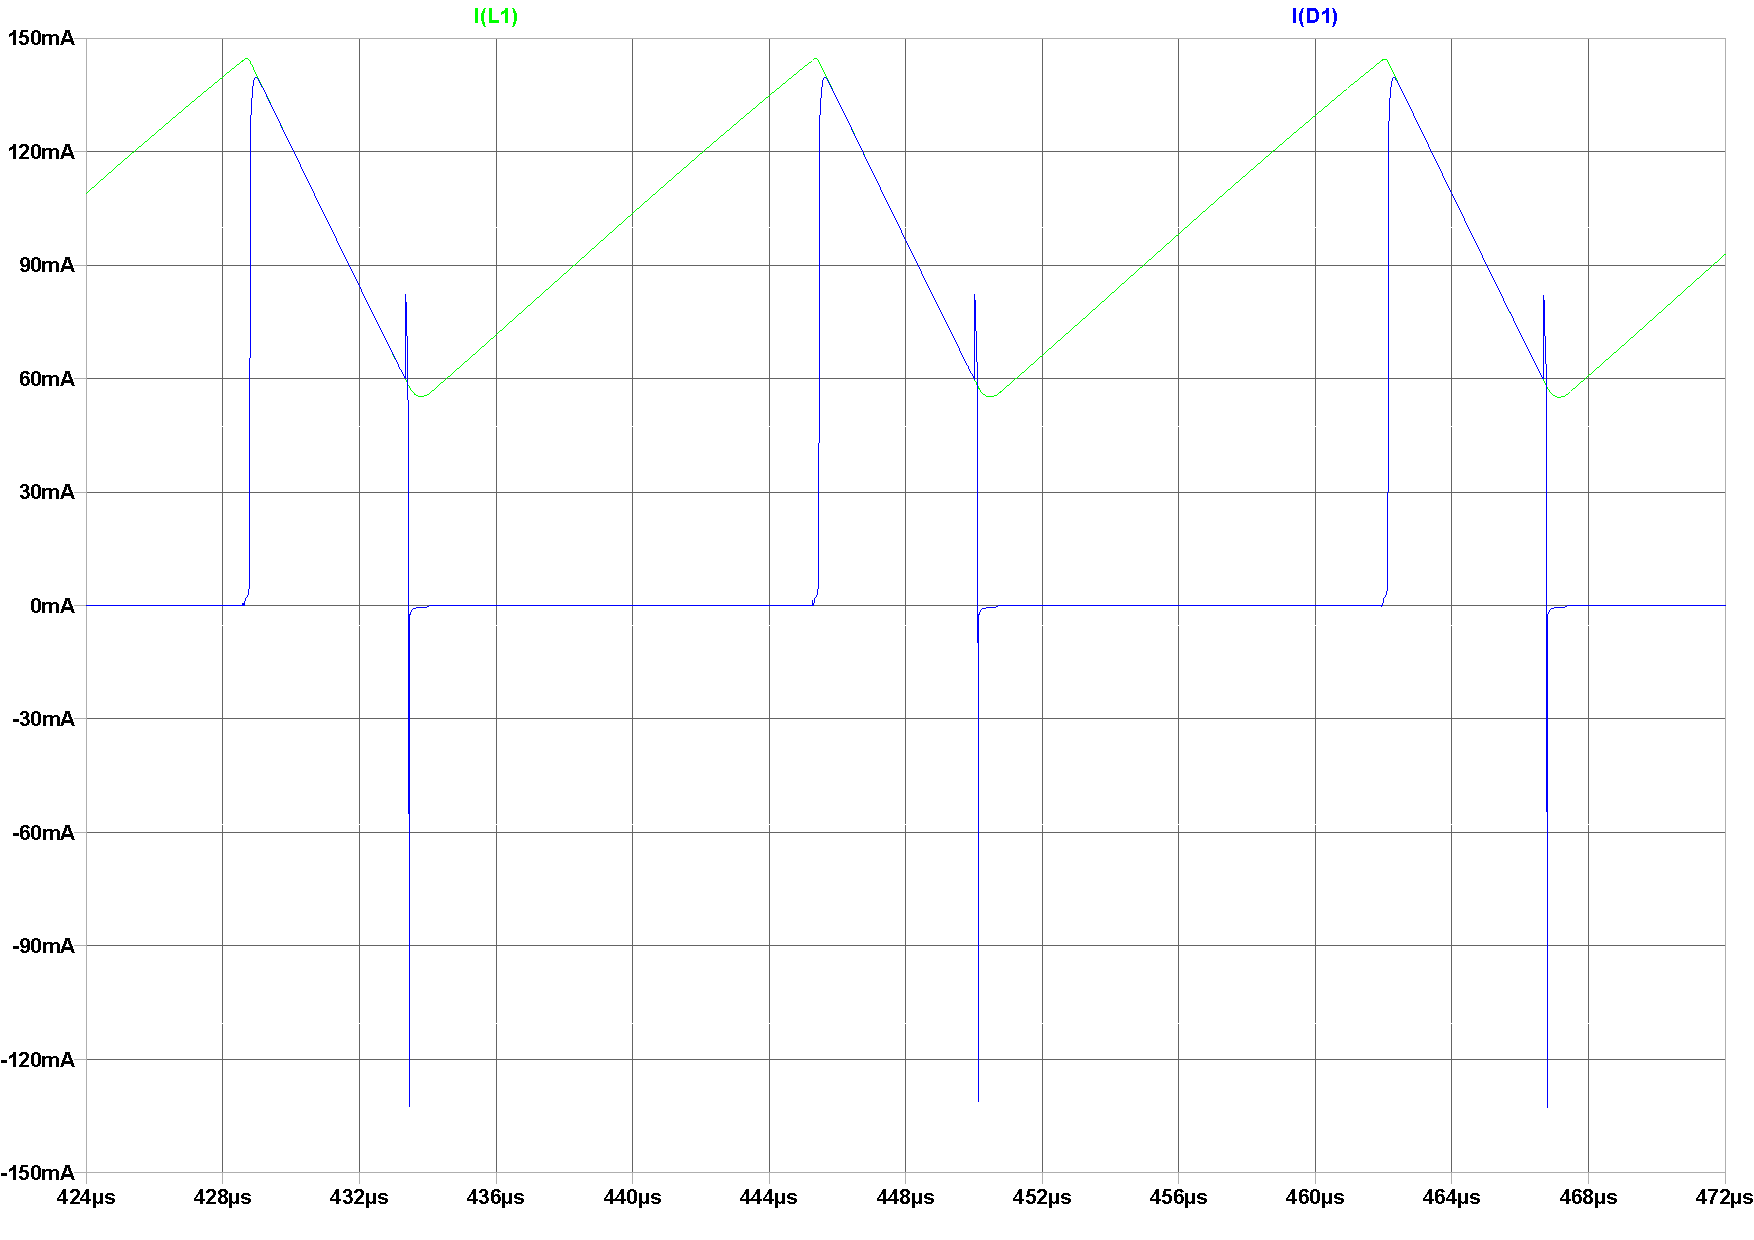
\includegraphics[width=0.8\linewidth]{Imagenes/Punto3/ID-IL.pdf}
\caption{Simulación ID(azul) y IL(verde)}
\end{figure}

\begin{figure}[H]
\centering
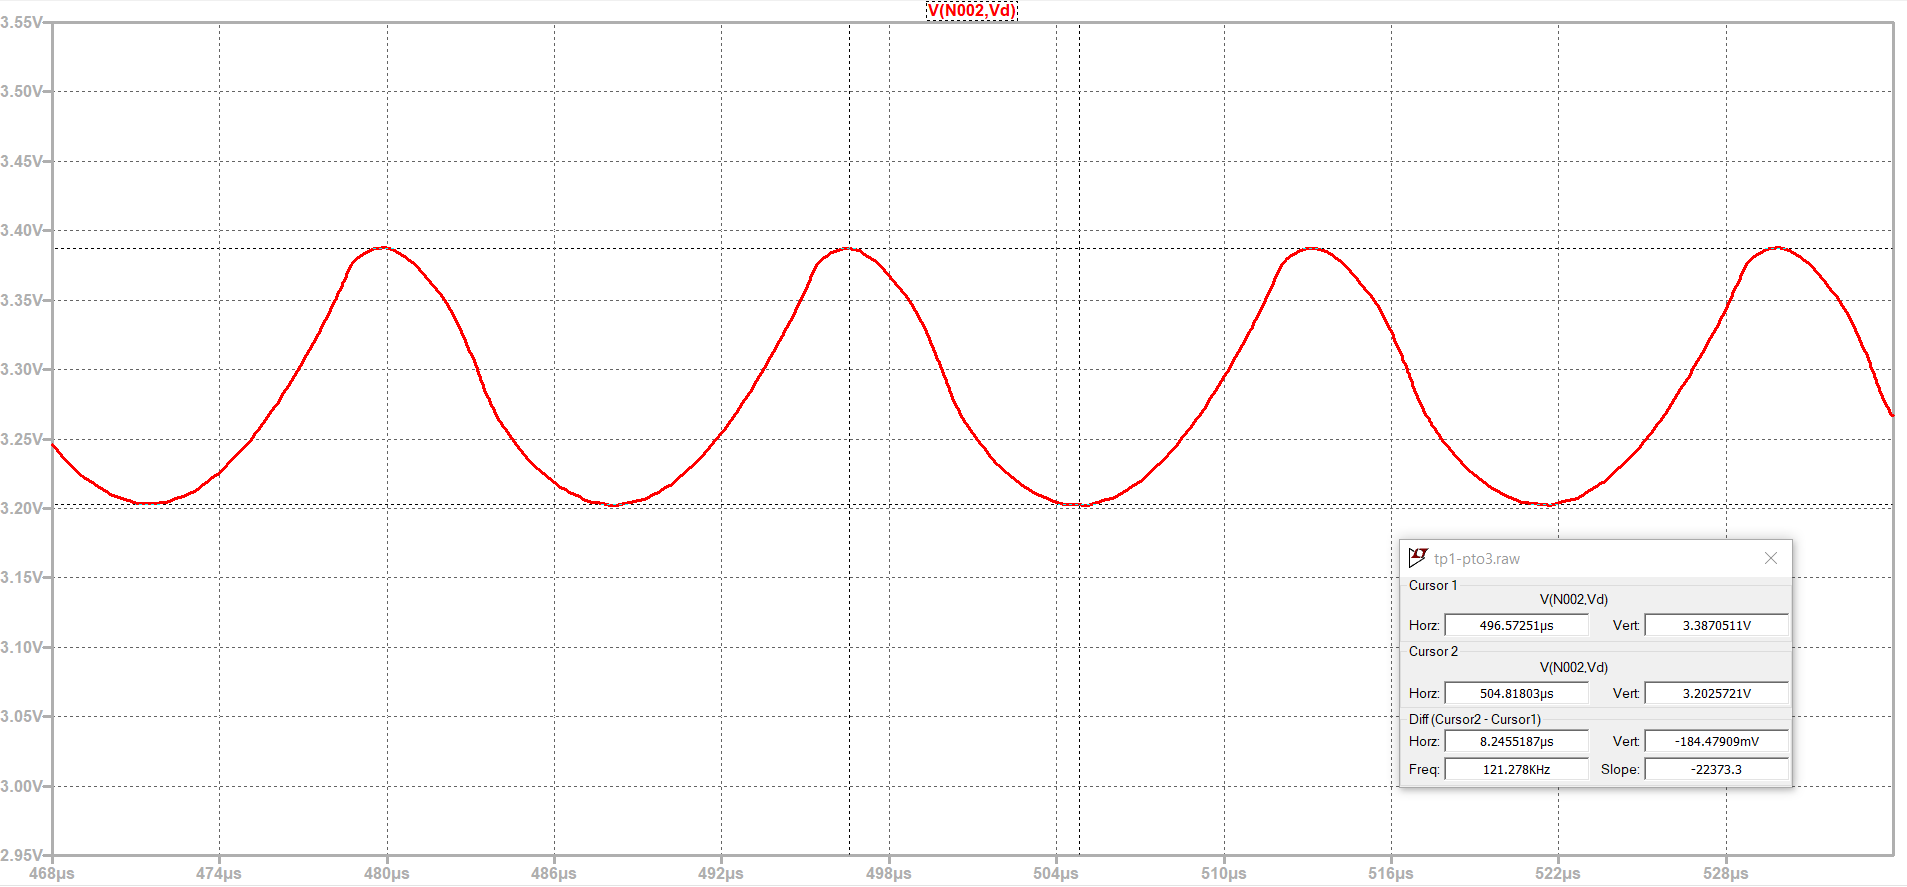
\includegraphics[width=1\linewidth]{Imagenes/Punto3/Vo.png}
\caption{Simulación salida $V_o$}
\end{figure}

\subsubsection*{1- Comparaciones y observaciones}

En las curvas simuladas se observa como afectan de igual forma los factores mencionados en la sección 2 con la fuente ideal.\par
La tensión sobre el drain, cuando el canal no conduce, equivale a la de la fuente más la caída de $V_{forw}$ en el diodo, que en el caso ideal no se tenía en cuenta. Mismo la tensión en la bobina alcanza los $4V$, que menos la caída del diodo se obtiene la salida la $V_o$ buscada. Cuando el canal conduce, sobre la bobina se tiene, en efecto, $V_d-V_o$.
\par
En el contraste de $I_D$ e $I_L$, se logra apreciar mejor el pico de corriente $I_{rr}$ del diodo al apagarse cuando el canal comienza a conducir, que en el gráfico de curvas de conmutación mostrado antes. En efecto, mientras el diodo conduce, la corriente que pasa a través de él es la misma que la de la bobina.
\par
El ripple obtenido es de $184mV$, que equivale a un $5,5\%$, un poco mayor al esperado.
\par
En cuanto a la potencia disipada en la llave, podemos observar que la misma queda expresada de la siguiente manera:\par
\[ 
P_{dis} = \frac{V_{in}*I_0*t_{conm}*f_{sw}}{2} = 13,23 mW  \] 
Esta potencia disipada representa el 2,65\% de la potencia total que entrega la fuente $V_d$.

\newpage
\end{document}